\subsection{Story: The Admin can show the results of the question in a sensible format e.g. graph}
\subsubsection{Analysis - breakdown of tasks}
\begin{itemize}
	\item Save the data
	\item Ensure no users submit twice
	\item Read from that data in the admin panel
	\item Prettify this results tab
\end{itemize}
\subsubsection{Design}
TODO: add initial design images here of the admin panel
\begin{figure}
	\caption{Use case for front end now including show results}
	\centerline{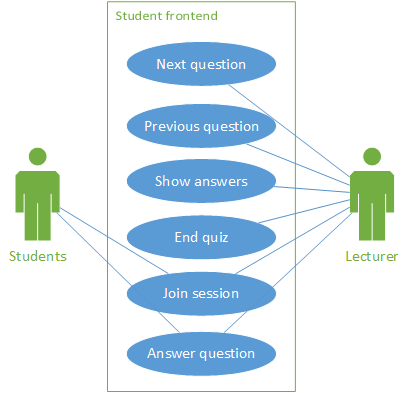
\includegraphics{Chapter2/Iter-6/iter-6-frontend-use-case}}
	\label{fig:iter-6-frontend-use-case}
\end{figure}
\subsubsection{Implementation}
There was quite a lot of work to do in this story, the first item in particular was the majority of work. At first it was decided that a simple database could be used to store all the responses however it was soon realised that users could probably submit more than once if we don't associate users with a response. The best way to deal with users that don't login is to use the Laravel session cookie to identify them anonymously.

To store all these responses in a database would be quite a lot of data, rather than having say six rows for a question with six answers that just tallies up the answers the actual session name had to be stored with the answer given so it could be changed. This meant that now there would be a row per answer, equalling at worst case 300 rows per question. This was thought to be a bit drastic so an alternative was suggested: to use a CSV file with each row having the user and an answer, with each question being a separate csv file. These would be stored locally under a session folder in the public directory. These files would be created and destroyed during quiz cycle. This method would also be a good for the downloading of answers from another story. 

Ultimately however, trying to write all this data to a csv was too troublesome to be worth it. If a user changed their answer then the entire csv had to be copied with one line changed, editing a single line is not possible with PHP. Therefore it was decided that going back to a database based method would be better, with the idea that at the end of a quiz, all the data would be deleted.

An answers table was created that specified the session, question, user and the answer given. The first three of those were used in a unique composite key to prevent multiple answers from the same users on the same questions in the same session. The model was then written to save this data when data was POST'ed to the /results url. Other functions include those to delete the data when a quiz was ended and various association functions.

To read this data on the front end, an AJAX request was set up from an admin panel button that GETs the same results url which calls an action to render the results data in a JSON format. The results are in a very basic format in a key-value pairs of answer, total number of selections.

This JSON data could then be used in the ChartJS library which was selected to render the results bar chart on the page\cite{chartjs}. The ChartJS library allows the creation of an object that can be attached to an HTML canvas tag. Within this object, the options and variables that make it up can be specified using JSON. The JSON data is split into two arrays of equal length, one of the keys and one of the values, they are then passed to the chart object and the results are rendered as a bar chart. This chart is then deleted if it already exists and rendered when the results button is pressed. This means every time it is pressed, the most up to date results will be displayed. 
\subsubsection{Testing}
Two things were tested here, the first is that users can submit their answers and that they are saved correctly in the database. The second is the testing how the results are shown by an admin.

For users submitting tests:
\begin{itemize}
	\item Test a student submitting a multiple choice answer
	\item Test a user changing their answer and resubmitting
	\item Test multiple users answering the same answer
	\item multiple students answering different answers
\end{itemize}

For the second task, testing the showing of results is relatively hard as the results box is rendered using an iframe and canvas HTML tags. It seems that anything within these cannot be seen by the assertions within Laravel Dusk and therefore cannot be reliably tested. A single test was written to check whether or not the iframe was made visible when the results button was clicked.
\newpage

\subsection{Story: Users should not be able to submit their own answers by altering the HTML, as they did with Qwizom}
\subsubsection{Analysis - breakdown of tasks}
Very few tasks as will be explained in the design subsection:
\begin{itemize}
	\item Add check for empty arrays on frontend
	\item Add check for empty arrays on backend
\end{itemize}
\subsubsection{Implementation}
Thanks to the design of the previous subsection, changing the data meant an empty key was sent if the user tried to change the data submitted to the server. This could be checked in either the JavaScript or PHP end, but it was decided both would be the best for maximum security. 
\subsubsection{Testing}
This is hard to test, as Dusk does not allow the changing of HTML on the page or the possibility to submit false data. Additionally, even if the data could be submitted the tests int he previous story indicate that the results cannot be read and therefore this story cannot be tested fully. User testing might be a good replacement for this.
\newpage

\subsection{Story: The Admin can see what percentage of users connected to the session have answered}
\subsubsection{Analysis - breakdown of tasks}
\begin{itemize}
	\item Get total number of responses
	\item Post this number on the page as part of the results form
\end{itemize}
\subsubsection{Design}
This should appear above the results table, possibly as part of the title.
\subsubsection{Implementation}
After attempting to get a number of users connected to the channel it became clear that this number is not readily accessible for public channels. It can be obtained via the Pusher API but implementing that would mean locking some functionality down with Pusher and the long term plan is likely to involve changing to a Redis based WebSocket system. Therefore this number has just been changed to the total number of responses which should give a good idea to the lecturer of what percentage of users have responded. This was simply added to the title attribute of the chart.
\subsubsection{Testing}
Like with the above stories this iteration, this cannot be tested because this information is contained within the iframe that cannot be seen in Dusk tests.
\newpage
